\documentclass[Main.tex]{subfiles}
\begin{document}
\section{Aanpak}
Aangezien de beperkingen van het \textit{Countdown probleem} niet van toepassing zijn, kunnen een groot deel van de gekende optimalisaties niet gebruikt worden. Als baseline wordt er gebruik gemaakt van een 'brute force algorithm'. Dit algoritme wordt vervolgens verbeterd door op een effici\"ente manier bepaalde vergelijkingen niet uit te rekenen of in het algemeen te vermijden.

\subsection{Brute Force}
Het 'brute force algorithm' bestaat uit twee delen die afwisselend worden uitgevoerd. Het eerste deel bestaat uit het uitbreiden van de bewerkingsboom (bv. de kinderen van de huidige knopen berekenen). In het tweede deel worden de bekomen vergelijkingen op elke mogelijke wijze ingevuld aan de hand van de productieregel die eindigt in een terminaal symbool. Bij elke volledige invulling van de knoop wordt deze berekend en vergeleken met het te behalen resultaat. Op deze manier moeten enkel de knopen die de gewenste oplossing hebben en de knopen die nog moeten worden uitgebreid bijgehouden worden. Dit zal enorm veel geheugen besparen. Hieronder zullen de twee stappen in meer detail overlopen worden. 

\subsubsection*{Het uitbreiden van de bewerkingsboom}
Het uitbreiden van de bewerkingsboom wordt bereikt door gebruik te maken van de context vrije grammatica uit Figuur \ref{fig:cfg}. De root van de bewerkingsboom $E$ wordt uitgebreid aan de hand van de regels van de contextvrije grammatica. De regel $E \rightarrow a | b | \dotsc$ wordt pas gebruikt bij het uitwerken van de vergelijkingen.

\subsubsection*{Het uitwerken van de vergelijkingen}
In deze stap wordt de regel $E \rightarrow a | b | \dotsc$ gebruikt om elke vergelijking in de bewerkingsboom een waarde te geven. Enkel deze regel wordt gebruikt en voor elke vergelijking wordt elke mogelijkheid afgegaan. Figuur \ref{fig:uitwerkingsboom} toont een gedeeltelijke uitwerking van de bewerkingsboom uit Figuur \ref{fig:vbBoom}.
\begin{figure}[!htb]
\centering
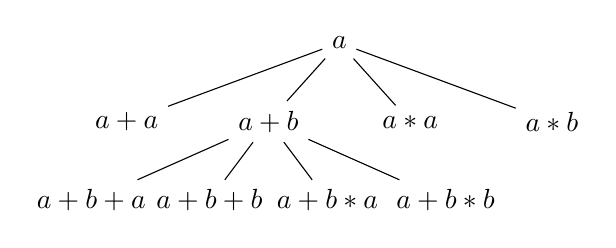
\begin{tikzpicture}[level distance=1cm,
  		level 1/.style={sibling distance=1.8cm},
  		level 2/.style={sibling distance=1.5cm}]
  		\node {$a$}
    		child {node {$a+a$}}
    		child {node {$a+b$}
    		    	child {node {$a+b+a$}}
    			child {node {$a+b+b$}}
    			child {node {$a+b \ast a$}}
    			child {node {$a+b \ast b$}}
    		}
    		child {node {$a \ast a$}}
		child {node {$a \ast b$}};
\end{tikzpicture}
\caption{Uitwerking bewerkingsboom (1 knoop per niveau)} \label{fig:uitwerkingsboom}
\end{figure}

\subsubsection*{Het resultaat}
Zolang er vergelijkingen gezocht worden waarin er zich geen constanten bevinden, bepaalt dit algoritme altijd een oplossing indien deze bestaat in de taal van de grammatica. Dit algoritme is zeer ineffici\"ent, zeker naarmate het aantal kolomwaarden toeneemt. 

\subsection{Toevoegen van constanten}
Het doel van het algoritme is dat er een vergelijking gevonden wordt die de gebruiker verlangt. Om een vergelijking zoals $2 \ast x+1$ te kunnen bepalen moeten er ook constanten toegelaten worden. Om hieraan te voldoen moet er slechts \'e\'en wijziging gebeuren in het vorige algoritme. Tijdens de uitwerking van de vergelijkingen moet de regel $E \rightarrow 1 | 2 .. 9 | a | b | \dotsc$ gebruikt worden in plaats van $E \rightarrow a | b | \dotsc$.

\subsubsection*{Het resultaat}
Door het toevoegen van constanten neemt de breedte van de uitgewerkte bewerkingsboom sterk toe. Bijgevolg stijgt de uitwerkingstijd, maar ook de oplossingsgraad stijgt als gevolg hiervan. De optimale verhouding tussen deze twee wordt bereikt door de keuze van de juiste constanten. Om de juiste keuze te kunnen maken zijn er experimenten uitgevoerd met verschillende sets van constanten. In sectie  \ref{ssec:constanten} wordt duidelijk gemaakt waarom de set ${1, 2, 3, 5, 7}$ wordt gekozen. Als baseline voor het optimaliseren van dit proces zal het 'brute force algorithm' met de set ${1, 2, 3, 5, 7}$ als constanten gebruikt worden.

\subsection{Prunen} \label{ssec:Prunen}
\subsubsection*{Prunen in de bewerkingsboom}
In de bewerkingsboom van het 'brute force algorithm' staan knopen die bij uitwerking altijd hetzelfde resultaat zullen opleveren. Een knoop $E$ is redundant als en slechts als er een knoop $E'$ bestaat die door toepassing van commutativiteit en rekening houdend met de volgorde van bewerkingen omgevormd kan worden tot $E$. Knopen die altijd hetzelfde resultaat opleveren zijn voorbeelden van redundante knopen (bv.  $E \ast E+E+E$ en $E+E \ast E +E$). Van sommige redundante knopen zijn ook al de kinderen redundant. Indien dit soort knopen verwijderd wordt, moeten de kinderen dus niet meer worden uitgerekend. Een voorbeeld van twee knopen die ook dezelfde kinderen hebben is: $E+E \ast E+E$ en $E \ast E+E+E$. Er bevinden zich ook knopen in de bewerkingsboom waarvan de kinderen niet exact dezelfde zijn maar de ouders wel. Een voorbeeld hiervan is het volgende: $E \ast E+E$ en $E+E \ast E$. De kinderen zijn niet redundant omdat de ouderknoop steeds rechts wordt uitgebreid. Een kind van $E \ast E+E$ is bijvoorbeeld $E \ast E+E \ast E$. Dit kind zal nooit een kind zijn van $E+E \ast E$. Er zijn verschillende momenten wanneer er in het algoritme gepruned kan worden. Deze zullen in de subsecties hieronder worden aangehaald.

\subsubsection*{Het op voorhand berekenen van de bewerkingsboom}
Het zoeken van redundante knopen vraagt tijd. De bewerkingsboom verandert niet zolang de contextvrije grammatica niet wijzigt. De mogelijkheid bestaat dus om de boom \'e\'enmalig op voorhand op te stellen en hierin te prunen. Op deze manier wordt de overhead van het prunen in de bewerkingsboom geminimaliseerd. Een nadeel aan deze optie is dat het prunen van de uitgewerkte boom (zie volgende sectie) tijdrovender wordt. Uit experimenten blijkt dat de tijdswinst van het op voorhand berekenen niet opweegt tegenover het tijdsverlies. Dit komt voornamelijk doordat de tijdswinst op lage niveaus in de bewerkingsboom ($< 8$) niet groot is en er verwacht wordt dat de gebruiker geen vergelijkingen zoekt van lengte groter dan 6. Het zal uit experimenten ook blijken dat vergelijkingen van lengte 6 en groter te veel tijd vragen om te berekenen. 

\subsubsection*{Prunen in de uitwerking van de bewerkingsboom}
In de uitwerking van de bewerkingsboom komen er redundante vergelijkingen naar boven. Zo zal de vergelijking $E+E-E$ in sommige gevallen redundant worden, bijvoorbeeld wanneer ze wordt vervangen door $a+a-a$. Ze is echter niet altijd redundant. Ze kan namelijk ook vervangen worden door $a+a-b$. Wanneer er vanuit gegaan wordt dat er constanten in de uitwerking voorkomen, onstaan er nog meer redundanties. Zo zal de vergelijking $E+E$ ook terug te vinden zijn als $2*E$. Dit wordt bereikt door bij de invulling van de waarden in de knopen het niet meer toe te laten dat een waarde met zichzelf gecombineerd wordt. Door deze redundante vergelijkingen effici\"ent te bepalen en deze niet uit te werken, kan er veel tijd bespaard worden.

\subsubsection*{Prunen in realiteit}
Het is mogelijk om alle redundanties te verwijderen zonder de oplossingsgraad te verlagen. Dit proces vraagt veel rekenwerk en bijgevolg veel tijd. Daarom is er gekozen om sommige redundanties niet te verwijderen (hieronder aangegeven als -), sommige te bewaren (hieronder aangegeven als +) en andere op  een meer eenvoudige wijze uit te werken (hieronder aangegeven als $\ast$). Dit laatste puntje zorgt er echter voor dat er ook niet redundante knopen zullen verloren gaan, bijvoorbeeld $a+1+1$ kan vervangen worden door $a+2$. Echter vraagt het zoeken van deze redundantie veel tijd. Algemener kan er gezegd worden dat er slechts \'e\'en losstaande constante mag voorkomen. Het nadeel hiervan is dat het aantal constanten beperkt is, en bijvoorbeeld de vergelijking $a+100$ verloren zal gaan. De focus van deze paper ligt op het voldoen aan de verwachtingen van de gebruiker. Daarom is in dit geval tijdswinst belangrijker dan een lichte daling in oplossingsgraad. 

\subsubsection*{Opsomming prunemogelijkheden} \label{ssec:pruningregels}
\begin{itemize}
\item[+] Een knoop wordt niet toegevoegd als de knoop en al zijn kinderen redundant zijn.
\item[+] Bij commutatieve operaties tussen waarden $a$ en $b$, moet gelden dat $a \geq b$.
\item[+] Bewerkingen die voorgaande bewerkingen ongedaan maken, maar enkel indien de termen exact dezelfde zijn.\\
	bv. $a*c+b-a*c$ valt weg, maar $a+a-2*a$ zal blijven bestaan
\item[+] Operaties met hun eenheidselement worden niet uitgerekend.
\item[-] Een knoop wordt toegevoegd als de knoop zelf redundant is maar zijn kinderen dat niet zijn.
\item[$\ast$] Constante waarden komen niet in combinatie met elkaar voor
\item[$\ast$] Niet toelaten van wiskundig equivalente termen
\end{itemize}

\end{document}